\SACCMD{transfer}
\label{cmd:transfer}

\SACTitle{概要}
反卷积以去除仪器响应,如果需要,还可以卷积其他仪器响应

\SACTitle{语法}
\begin{SACSTX}
TRANS!FER! [FROM type [options]] [TO type [options]]
    [FREQ!LIMITS! f1 f2 f3 f4] [PREWH!ITENING! ON|OFF|n]
\end{SACSTX}

\SACTitle{输入}
\begin{description}
\item [FROM type] 要去除的仪器响应类型;
\item [TO type] 要加入的仪器响应类型;
\item [FREQLIMITS f1 f2 f3 f4] 压制大于f4以及低于f1的频段;
\item [PREWHITENING ON|OFF|n] 预白化处理。
\end{description}

\SACTitle{缺省值}
\begin{SACDFT}
trans from none to none
\end{SACDFT}

\SACTitle{说明}
\subsubsection{FROM and TO}
transfer命令的作用是将波形数据从一种仪器响应转换成另一种仪器响应。
\texttt{FROM type} 指定要从波形数据中去除的仪器响应,\texttt{TO type} 指定了要加入
到波形数据中的仪器响应。去仪器响应即反卷积,加仪器响应即卷积,二者分别通过
谱域的除法和乘法完成。

\texttt{type} 为仪器类型,可以是SAC预定义的标准仪器类型
(见附录中表 \ref{table:instrument-type}),还可以是如下几种特殊的``仪器类型'':
\begin{description}
\item [none] 表示``位移''
\item [vel] 表示``速度''
\item [acc] 表示``加速度''
\item [evalresp] 表示使用RESP仪器响应文件
\item [polezero] 表示使用SAC PZ仪器响应文件
\item [fap] 表示使用fap仪器响应文件
\end{description}

tranfser命令的默认值是``\texttt{transfer from none to none}'',即默认的输入和
输出``仪器''都是位移。因而当不指定 \texttt{FROM type} 或 \texttt{TO type} 时,SAC
会假定仪器类型为 \texttt{NONE}。

\begin{itemize}
\item 若输出的仪器类型为 \texttt{NONE},即表示从波形中去除仪器响应得到位移,
    此时SAC头段中的IDEP设置为 \texttt{IDISP},单位为 \texttt{nm},若输出类型为
    \texttt{VEL} 或 \texttt{ACC},同理;
\item 若输出的仪器类型不是 \texttt{NONE}、\texttt{VEL} 或 \texttt{ACC},则内存中的波形会
    卷积上 \texttt{TO type} 所指定的仪器响应;
\item 若不指定 \texttt{FROM} 选项,则假定原始波形数据是位移,且不会去除仪器响应;通常
    用于给理论地震图添加仪器响应;
\end{itemize}

\subsubsection{freqlimits}
freqlimits用于在去除仪器响应时对波形的低频和高频部分进行压制。当 \texttt{TO type} 为
NONE、VEL或ACC时,必须使用该选项,且必须认真选择合适的参数。

所有地震仪在零频率处都具有零响应,在只进行反卷积时,需要在频率域做谱的除法,此时
可能会除以一个很小的值进而导致低频处有很大的谱振幅;在高频处,信噪比通常很低,
因而有必要对其响应进行压制。

freqlimits会在去仪器响应时对频谱做低通和高通尖灭,以实现对高频和低频的压制。
四个频率参数应满足 \texttt{f1<f2<f3<f4},即尖灭函数在零到f1之间为0,f1到f2之间
从0渐渐变成1,在f2和f3之间保持为1,在f3到f4之间从1渐渐变成0,大于f4的频段
值为0。过渡带内分别为余弦波的四分之一周期。如下图所示:

\begin{figure}[H]
\centering
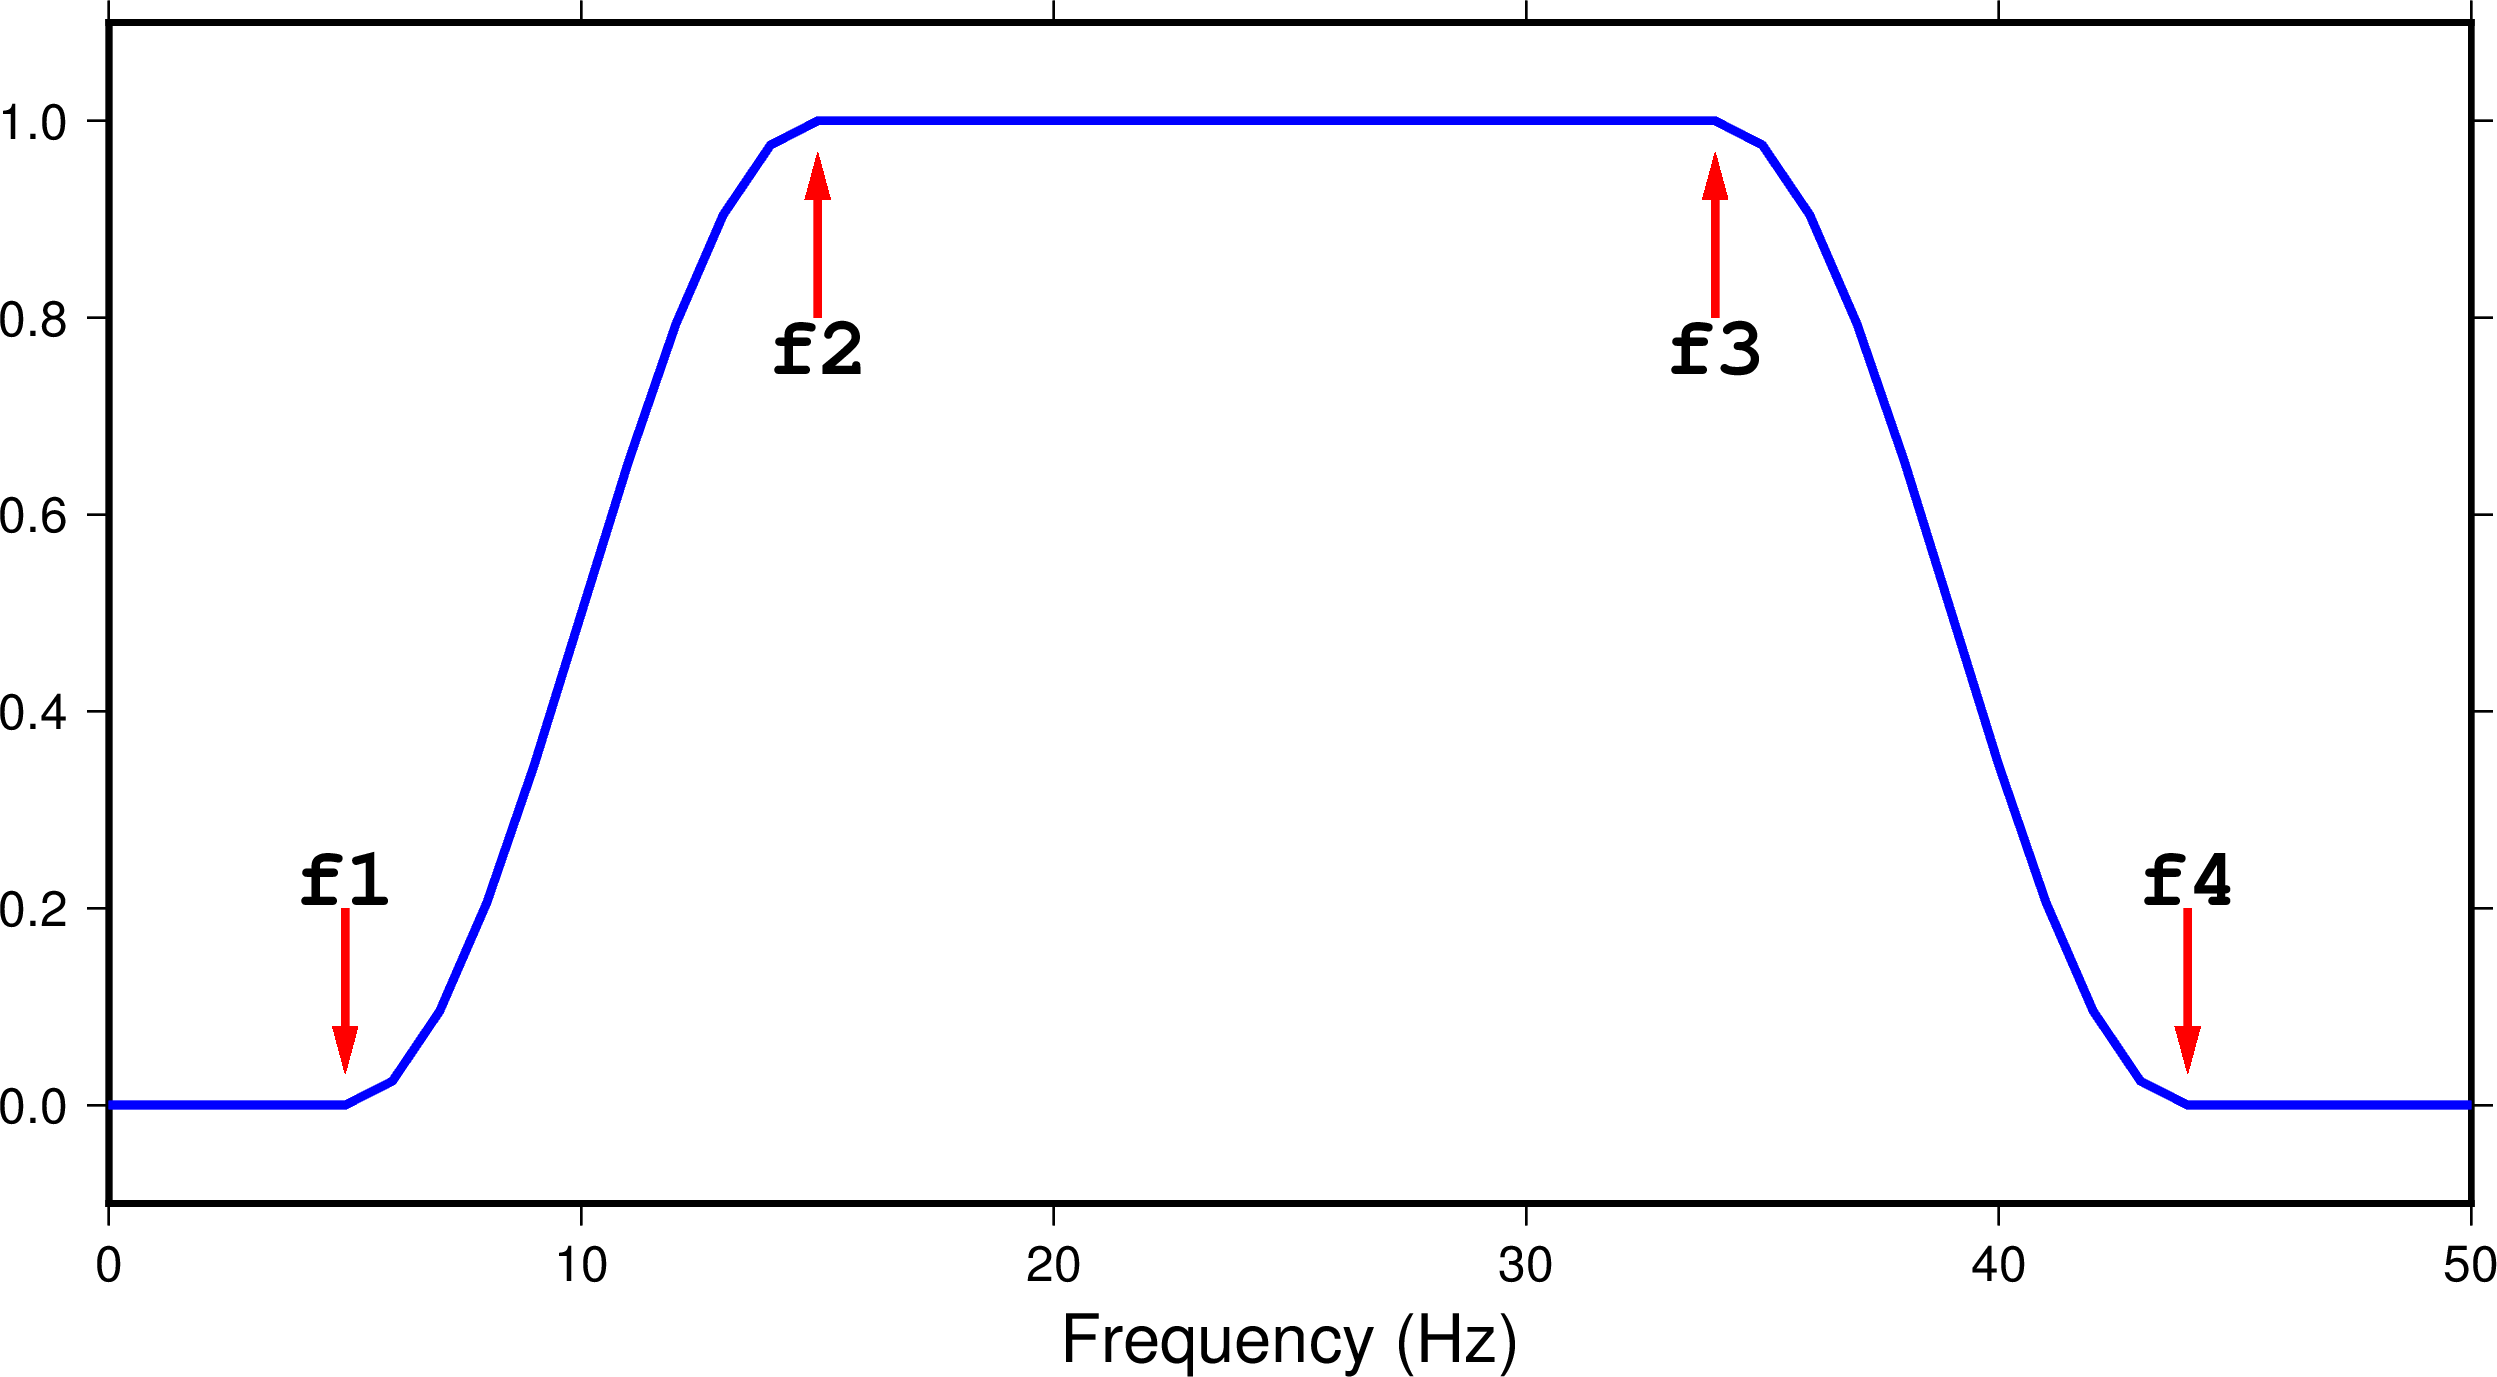
\includegraphics[width=0.9\textwidth]{freqlimits}
\caption{Freqlimits尖灭函数}
\label{fig:freqlimits}
\end{figure}

四个频率参数除了要满足 \texttt{f1<f2<f3<f4} 外,还应注意如下几条原则:
\begin{itemize}
\item \texttt{f4} 应小于Nyquist采样率。比如若数据的采样周期为 \SI{0.01}{\s},则Nyquist采样率
    为 \SI{50}{\Hz},因而f4应小于\SI{50}{\Hz};
\item f3不能与f4太接近;
\item f2与f3之间应尽可能宽,然后再根据具体需求进行滤波;
\item f1和f2不能太接近;
\item f1的选取由具体需求决定,可以尝试不同的值并查看去仪器响应之后的效果来决定;
\end{itemize}

若想要一个低通滤波器但在低频处不滤波,可以设置 \texttt{f1=-2} 和 \texttt{f2=-1} ;
若想要一个高通滤波器但在高频处不滤波,可以设置f3等于Nyquist频率,f4为Nyquist频率的两倍。

需要注意,该滤波器是零相位、非因果滤波器,因而,若数据点数不为2的指数幂次,
会导致在频段 \texttt{(f1,f4)} 之外振幅不完全为0。若想要数据点数为2的幂次方,
可以参考SAC中的 \nameref{cmd:cut} 命令。

\subsubsection{prewhitening}
\texttt{prewhitening} 用于控制数据的预白化。预白化可以将输入时间序列在变换到
频率域之前,进行谱的平化。这会减小谱值的动态范围,并提高数据在高频的计算精度。
参见 \nameref{cmd:whiten} 命令。打开预白化选项,会在谱操作之前在频率域进行谱白化,
并在谱操作后在时间域做谱白化的补偿,也可以设置预白化选项的阶数。默认情况下,
预白化选项是关闭的,阶数为 \texttt{n=6} 。

\SACTitle{示例}
\subsubsection{内置仪器类型}
SAC中内置了一堆预定义的仪器类型,可以在命令中直接使用。

从数据中去除LLL宽频带仪器响应。并卷积上SRO仪器响应,且对频带做尖灭及预白化:
\begin{SACCode}
SAC> read abc.z
SAC> rmean; rtr; taper
SAC> trans from lll to sro freq .02 .05 1. 2. prew 2
\end{SACCode}

当前的仪器类型为RSTN的子类型nykm.z,为了去除该仪器响应并卷积上DSS仪器响应:
\begin{SACCode}
SAC> read nykm.z
SAC> rmean; rtr; taper
SAC> trans from rstn subtype nykm.z to dss prew off
\end{SACCode}

将电磁仪器响应转换成位移:
\begin{SACCode}
SAC> r XYZ.Z
SAC> trans from elmag freep 15. mag 750. to none
\end{SACCode}

从波形中去除WWSP的仪器响应,得到位移波形:
\begin{SACCode}
SAC> read xyz.z
SAC> rmean; rtr; taper
SAC> trans from WWSP to none freq 0.05 0.01 5 10
                // 也可使用to vel或to acc得到速度或加速度
\end{SACCode}

向合成的位移地震图中加入WWSP仪器响应:
\begin{SACCode}
SAC> r syn.z
SAC> trans from none to WWSP    // 简写为trans to WWSP
\end{SACCode}

\subsubsection{evalresp类型}
\texttt{evalresp} 类型并不代表真正意义上的仪器类型,而是表示从RESP仪器响应文件中
读取仪器响应信息。在使用 \texttt{evalresp} 选项时,\nameref{cmd:transfer} 依次从
当前内存中的SAC波形数据中提取出各自的头段信息,包括:\texttt{kstnm}、\texttt{kcmpnm}、
\texttt{kzdate}、\texttt{kztime}、\texttt{knetwk} 和 \texttt{locid},然后会在当前目录下
寻找文件名为``\texttt{RESP.<NET>.<STA>.<LOCID>.<CHN>}''的RESP文件(比如``RESP.IU.COLA..BHZ''),
并检测RESP文件中给出的台站信息是否与数据中的台站信息匹配
\footnote{即,要求RESP文件名以及RESP文件中的台站信息都与数据头段中的台站信息匹配}。
\begin{SACCode}
SAC> r 2006.253.14.30.24.0000.TA.N11A..LHZ.Q.SAC
SAC> rtr; rtr; taper
SAC> trans from evalresp to none freq 0.004 0.007 0.2 0.4
\end{SACCode}
该命令会首先从头段中提取台站信息,然后自动在当前目录下寻找文件 \texttt{RESP.TA.N11A..LHZ},
一旦文件中的台站信息与数据中的台站信息匹配,则使用该响应函数。

SAC数据中的头段信息可以用一些选项来覆盖:
\begin{verbatim}
    STATION, CHANNEL, NETWORK, DATE, TIME, LOCID, FNAME
\end{verbatim}
每个选项都必须有一个合适的值。若DATE在SAC头段中未设定且在选项中未指定,
则使用当前系统日期,TIME同理;若NETWORK未指定,则默认使用任意台网名;
若LOCID或KHOLE未指定,则默认使用任意LOCID。

假设台网IU的所有台站都具有完全相同的仪器响应函数,而此时我们只有COLA台站的RESP
文件``RESP.IU.COLA..BHZ''。为了给所有台站去除仪器响应,一种办法是对IU台网的每一个
台站复制一份``RESP.IU.COLA..BHZ'',重命名,并修改RESP文件中的台站信息。显然,这样
很麻烦,利用上面的选项可以大大简化这一过程:
\begin{SACCode}
SAC> r *.IU.*.BHZ
SAC> rmean; rtr; taper
SAC> trans from evalresp STATION COLA to none freq 0.01 0.02 5 10
\end{SACCode}
使用STATION选项覆盖了波形数据中的台站名,此时,对每一个波形数据,transfer命令都会
去使用``RESP.IU.COLA..BHZ''\footnote{这里假定所有台站的LOCID都是未定义的}。

下面的命令会将三分量数据去仪器响应,并卷积上BHZ分量的仪器响应:
\begin{SACCode}
SAC> r *.IU.COLA.00.BH?
SAC> rmean; rtr; taper
SAC> trans from evalresp to evalresp CHANNEL BHZ
\end{SACCode}
操作完成后,BHZ分量相当于没有进行操作,BH1和BH2则去除了原本的仪器响应并卷积上BHZ的
仪器响应。

为了显示IU台网COL台站BHZ通道,1992年01月02日16:42:05的仪器响应:
\begin{SACCode}
SAC> fg impulse npts 16384 delta .05 begin 0.
SAC> trans to evalresp sta COL cha BHZ net IU \
                    date 1992/2 time 16:42:05
SAC> fft
SAC> psp am
\end{SACCode}

如果你的RESP文件名与SAC的标准格式不同,可以使用FNAME选项强制指定要使用的RESP文件:
\begin{SACCode}
SAC> r 2006.253.14.30.24.0000.TA.N11A..LHZ.Q.SAC
SAC> rmean; rtr; taper
SAC> trans from evalresp fname /tmp/Resp/RESP.TA.N11A..LHZ to none \
                        freq 0.004 0.007 0.2 0.4
\end{SACCode}
transfer命令默认会使用``RESP.TA.N11A..LHZ''作为响应文件,此处使用FNAME选项强制指定
使用``/tmp/RESP/RESP.TA.N11A..LHZ''。需要注意的是,即便是使用FNAME强制指定了RESP文件,
该命令还是会检测台站信息是否匹配。

由于一个RESP文件中可以包含多个响应函数,因而可以将所有仪器响应文件合并到一个总的
RESP文件中:
\begin{SACCode}
SAC> r *.SAC
SAC> rmean; rtr; taper
SAC> transfer from evalresp fname RESP.ALL to none freq 0.1 0.2 5 10
\end{SACCode}
这个例子中,RESP.ALL包含了所有数据的响应函数,transfer命令会读取RESP.ALL文件的内容,
对于每一个波形数据,会从波形数据中提取出台站信息,并与RESP.ALL中的众多响应函数进行
匹配,若匹配成功,则使用该响应函数。

\subsubsection{polezero类型}
\texttt{polezero} 类型并不代表真正意义上的仪器类型,而是表示从SAC零极点文件中读取仪器
响应函数。

polezero类型会从数据波形中提取台站信息,但不会根据台站信息去寻找默认的PZ文件,用户
必须使用 \texttt{subtype} 来指定要使用的PZ文件。若PZ文件有注释行,则注释行中的台站信息
必须与波形中的台站信息匹配,才能正确执行;若PZ文件中无注释行,则不进行台站信息匹配
的检测,直接执行。
\begin{SACCode}
SAC> r *IU.COLA.BHZ
SAC> rmean; rtr; taper
SAC> trans from polezero subtype SAC_PZs.IU.COLA.BHZ to WWSP
\end{SACCode}

一个PZ文件中可以包含多台站、多通道、多时间段的响应函数。可以将所有数据的PZ
文件合并得到总的PZ文件。下面的例子中读入全部波形数据,并利用总PZ文件进行去
仪器响应:
\begin{SACCode}
SAC> r *.SAC          // 读入全部数据
SAC> rmean; rtr; taper
SAC> trans from polezero s event.pz to none freq 0.05 0.1 10.0 15.0
SAC> mul 1.0e9        // 需要乘以1.0e9 !!!!!
SAC> w over
\end{SACCode}

需要格外注意,在用PZ文件去仪器响应得到位移物理量时,得到的数据的单位是 \texttt{m},
而SAC中默认的单位是 \texttt{nm},因而需要将数据乘以 \texttt{1.0e9} 将数据的单位
转换成 \texttt{nm}。对于转换得到速度或加速度,同理。

\subsubsection{fap选项}
fap选项表明使用FAP文件作为响应函数。

假设有fapfile文件 \verb|fap.n11a.lhz_0.006-0.2|,其名字表示频率段为0.006 Hz到0.2 Hz,
要从波形 \texttt{2006.253.14.30.24.0000.TA.N11A..LHZ.Q.SAC} 中移除该仪器响应:
\begin{SACCode}
SAC> r 2006.253.14.30.24.0000.TA.N11A..LHZ.Q.SAC
SAC> rtr
SAC> taper
SAC> trans from fap s fap.n11a.lhz_0.006-0.2 to none \
                        freq 0.004 0.006 0.1 0.2
SAC> mul 1.0e9
\end{SACCode}
